\chapter{初段ミューオントリガーの性能評価}\label{chapter5}
本章では、\ref{chapter4}で述べた手法で作成した2種類の CW (シミュレーション用の CW と実際の測定用の CW) を用いたトリガーの性能の評価を行う。
便宜上、本手法で作成した 2 種類の CW について、シミュレーション用の CW を $\mathrm{CW_{Simu}}$、実際の測定用の CW を $\mathrm{CW_{Data}}$ と呼び、2022年 Run-3 で使用された CW を $\mathrm{CW_{2022}}$ と定義する。

\section{機械学習で作成した CW を用いたトリガーの性能評価}
\subsection{評価方法}
トリガー効率$\epsilon$について式\ref{equ:Eff}を用いて評価を行う。
ここで、全ミューオン数はTGC にヒットした全オフライン再構成されたミューオンと定義し、その中でトリガーを発行したミューオンの数を調べ、トリガー効率を計算する。
このとき得られるトリガー効率を $p_T$ の関数で表したプロットを Turn-on curve と呼ぶ。
\begin{equation}
    \epsilon = \frac{ある p_T 閾値以上のトリガーを発行したミューオンの数}{全オフライン再構成したミューオンの数}
 \label{equ:Eff}
\end{equation}
定量的な評価のために\eqref{equ:fitting5}で定義する関数を用いてフィッティングを行う事で、トリガー性能の評価を行った。
\begin{equation}
    f(p_T) = \frac{p_0}{exp(\frac{p_T-p_1}{p_2})+1}
 \label{equ:fitting5}
\end{equation}
ここで\ref{section:fitting}節で述べたように、$p_0$は Plateau efficiency、$p_1$は Effective threshold、$p_2$は Resolution を表している。

\subsubsection{Tag$\&$Probe法}
実際の実験データはトリガーによって選別された粒子の情報のみが保存されているため、そのままのデータを用いてトリガーの性能評価や解析を行うとバイアスがかかる可能性がある。そこで解析の手法として Tag$\&$Probe 法を用いる。

Tag$\&$Probe 法では、一般的に Z ボゾン や J/ψ 粒子の崩壊で生じた 2 つのミューオンを使用する。2 つのミューオンのうち、片方のミューオン (Tag) が事象選択のトリガーとしてトリガーが発行された場合、もう一方のミューオン (Probe) をトリガー効率測定に用いる。Probe ミューオンに対してトリガーが発行されたかを見ることで, 実験でトリガーによって取得されたというバイアスをなくしてトリガー効率を見積もることができる。

本研究では、内部飛跡検出器とミューオン検出器でそれぞれ独立にオフライン再構成された Z ボソン由来のミューオンを用いて評価を行う。1回の衝突事象に対し、2 つ以上のミューオン候補が存在するイベントのみを用いる。それらのミューオン候補のうち、任意の2つの電荷が異符号となっているミューオンペアを選び出し、不変質量を再構成する。再構成の条件は、$80 GeV < M_Z < 100 GeV$ とする。
これらのミューオンのうち、一方を Tag ミューオン、もう一方を Probe ミューオンと定義する。
まず、Tag ミューオンがトリガーを発行したかどうかを判定する。Run-2 での実験データを解析に使用する際のトリガー判定には、HLT のシングルミューオントリガーである 「HLT$\_$mu26$\_$ivarmeduium」 を使用する。
ここでトリガー発行の判定を行うために $\Delta R = \sqrt{(\Delta \eta)2 + (\Delta \phi)2}$ を定義する。ここで $\Delta \eta$, $\Delta \phi$ はそれぞれデータの保存されているトリガーを発行した飛跡と Tag ミューオンの $\eta$ 方向、$\phi$ 方向の差である。図\ref{fig:tag_HLT}にTag ミューオンと HLT の $\Delta R$ 分布を示す。本研究では$\Delta R < 0.001$ を満たせば Tag ミューオンがトリガーを発行したとみなす。Tag ミューオンが HLT を発行しているとみなされた時、もう一つのミューオンを Probe ミューオンとして解析に使用する。

\begin{figure}[tb]
  \centering
  %\rule{8cm}{6cm}
  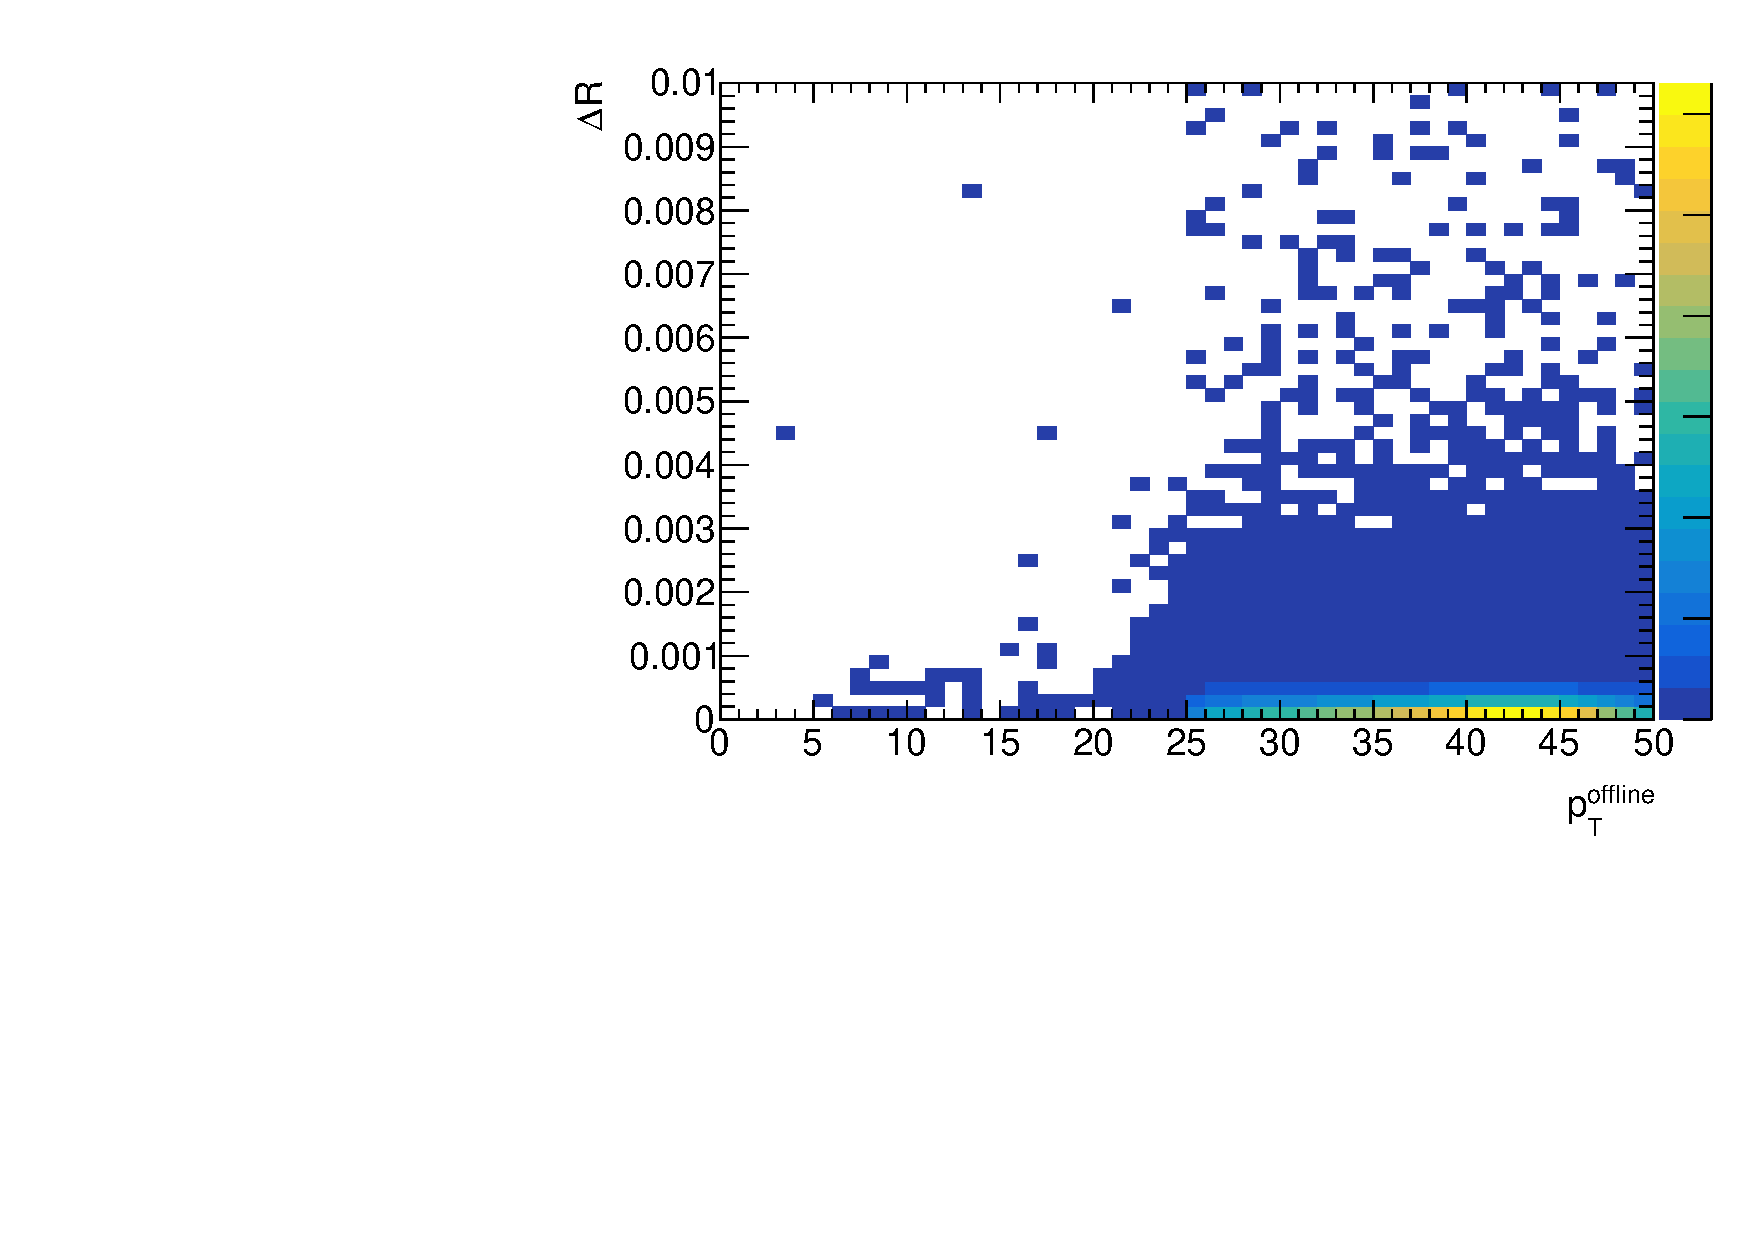
\includegraphics[clip, width=11cm]{fig/3/dR_tag_HLT.pdf}
  \caption{Tag ミューオンと HLT の $\Delta R$ 分布。$\Delta R < 0.001$ ならば Tag ミューオンが HLT を発行したものとする。}
  \label{fig:tag_HLT}
\end{figure}

Probe ミューオンは正しく再構成され、発行されたトリガーとは独立なミューオンである。
Probe ミューオンを使用してエンドキャプ部のトリガー性能を評価するために、Probe ミューオンと TGC のヒット情報を一致させる。図\ref{fig:Probe_TGC}に Probe ミューオンと TGC のヒット情報 の $\Delta R$ 分布を示す。本研究では$\Delta R < 0.04$ を満たせば Probe ミューオンが TGC のヒット情報と一致したものとする。
Probe ミューオンの情報とこのミューオンと一致したTGC のヒット情報を使って解析を行う。

\begin{figure}[tb]
  \centering
  %\rule{8cm}{6cm}
  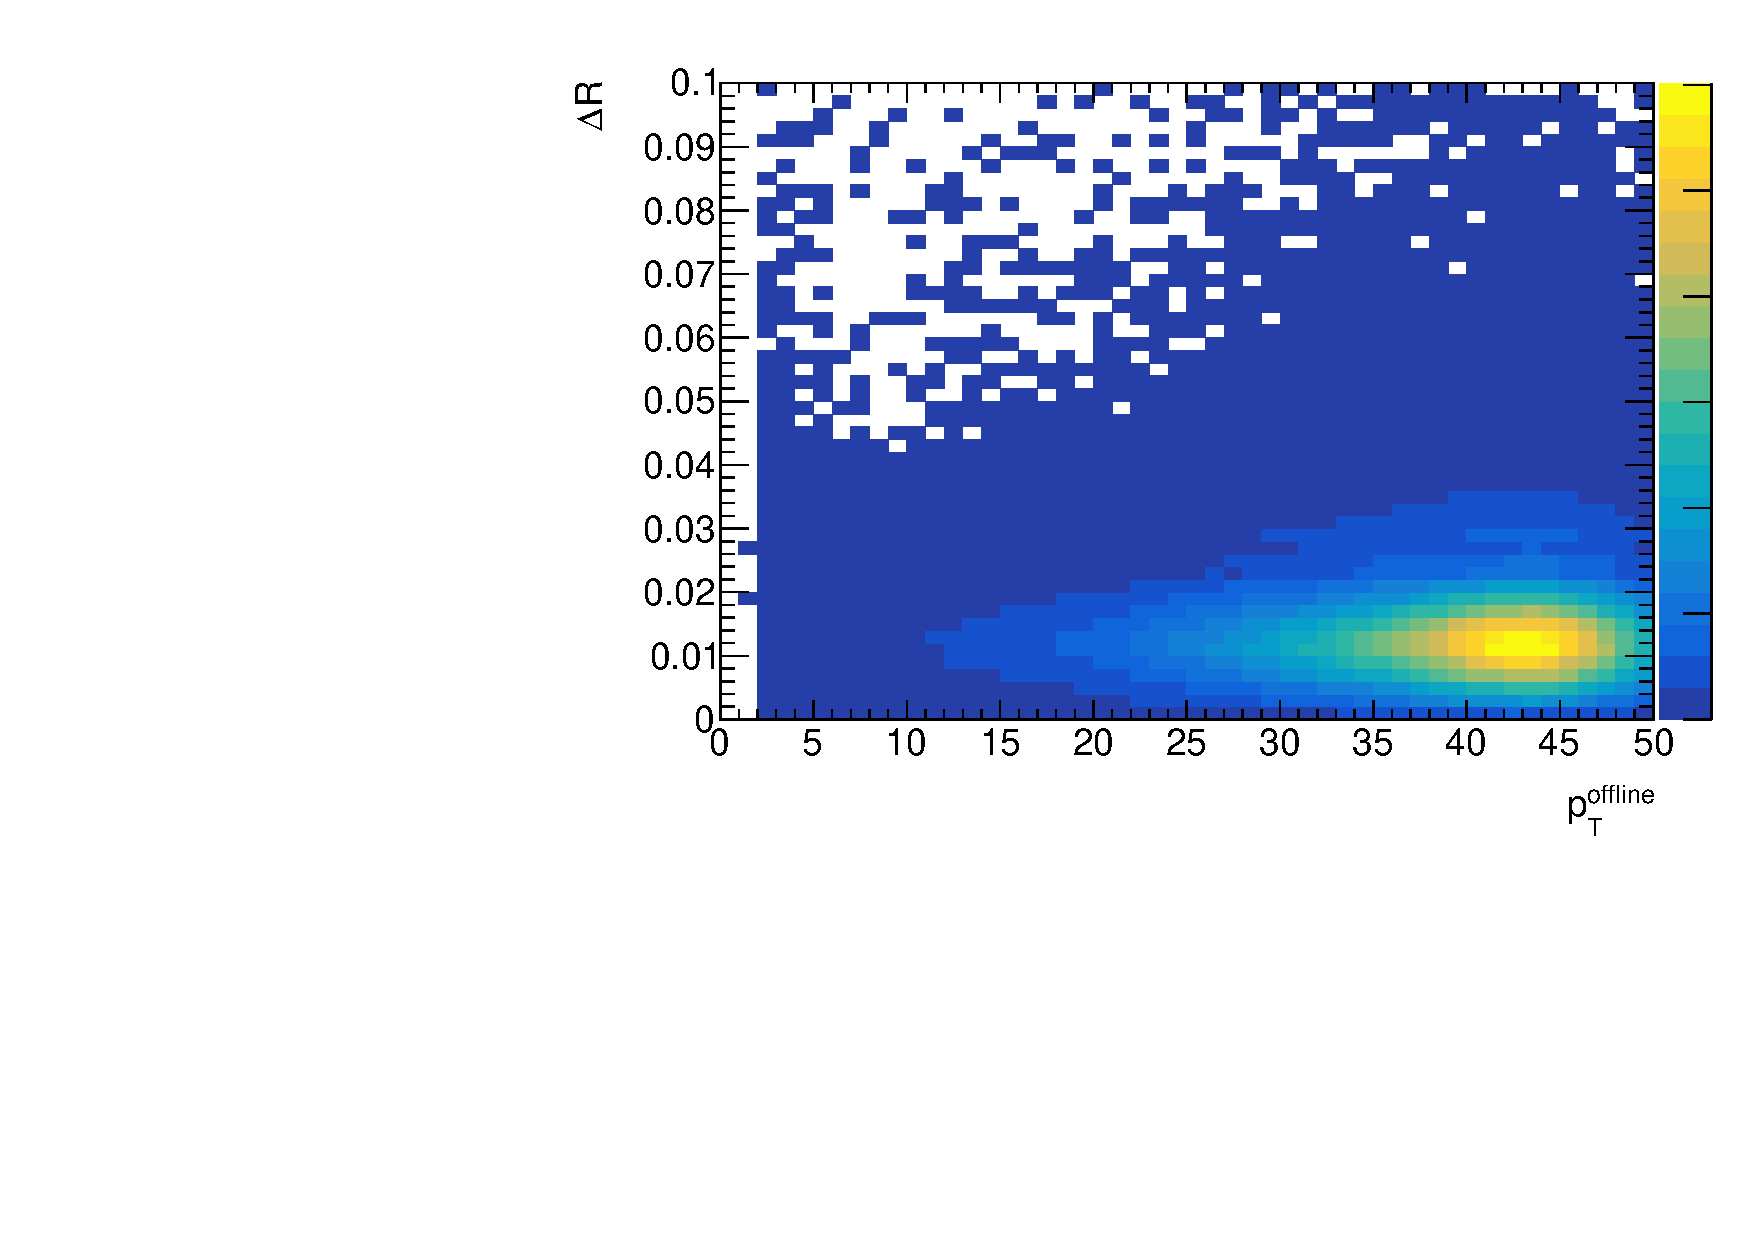
\includegraphics[clip, width=10cm]{fig/3/dR_probe_RoI.pdf}
  \caption{Probe ミューオンと TGC 1ヒット情報との $\Delta R$ 分布。$\Delta R < 0.04$ ならば Probe ミューオンが TGC のヒット情報と一致したものとする。}
  \label{fig:Probe_TGC}
\end{figure}

\subsection{機械学習を用いて作成した CW の 15 段階 $p_T$ 閾値}
Run-3 に向けて新たに作成した CW のトリガー効率の評価を行う。

$\mathrm{CW_{Data}}$ の図\ref{fig:15Eff_CW_Simu} に $\mathrm{CW_{Simu}}$ を用いて3 ステーションコインシデンスのみで hotroi フラグを要求した結果の15段階の $p_T$ 閾値における Turn-on curve を示す。$\mathrm{CW_{Simu}}$ の評価にはシングルミューオンのシミュレーションデータを用いた。
図\ref{fig:15Eff_CW_Data}に$\mathrm{CW_{Data}}$を用いて3 ステーションコインシデンスのみで hotroi フラグを要求した結果の15段階の $p_T$ 閾値における Turn-on curve を示す。評価には2018 年 Run-2 のデータに対して $Z \rightarrow \mu\mu$ による Tag $\&$ Probe 法を用いた。比較のため、図\ref{fig:Run3_15_MC5} に $\mathrm{CW_{2022}}$ の Turn-on curve を示す。

まず、2018年 Run-2 データを用いて本手法で作成した $\mathrm{CW_{Data}}$ と $\mathrm{CW_{Simu}}$ の比較を行う。図\ref{fig:v06v07}に同じ閾値の Turn-on curve を比較したプロットを示す。$\mathrm{CW_{Data}}$ の方が実際のデータに対してのトリガー効率が良くなっているのが見て取れる。これは、実際のデータを学習に使用したことで、検出器のズレに対応し、CW の最適化ができたことを示している。
\begin{figure}[tb]
  \centering
  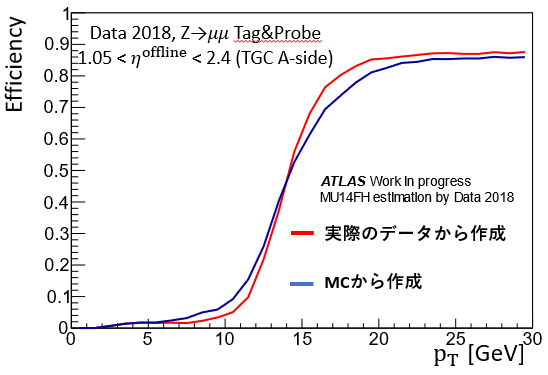
\includegraphics[clip, width=12cm]{fig/4/hikaku_v06_v07.png}
  \caption{v06v07}
  \label{fig:v06v07}
\end{figure}

次に、本手法で作成した $\mathrm{CW_{Data}}$ と $\mathrm{CW_{Simu}}$ を $\mathrm{CW_{2022}}$ と比較する。
図\ref{fig:v05v06} には $\mathrm{CW_{2022}}$ の各閾値と同程度のパフォーマンスでとなる $\mathrm{CW_{Simu}}$ の Turn-on curve を示し、図\ref{fig:v05v07} には $\mathrm{CW_{2022}}$ の各閾値と同程度のパフォーマンスでとなる $\mathrm{CW_{Data}}$ の Turn-on curve を示した。
各 Turn-on curve に\eqref{equ:fitting5}によるフィッティングを行い Turn-on curve の Resolitionvを比較する。図\ref{fig:Resolution_v07v05}に $\mathrm{CW_{Simu}}$ と $\mathrm{CW_{2022}}$ の比較、 図\ref{fig:Resolution_v06v05}に $\mathrm{CW_{Simu}}$ と $\mathrm{CW_{2022}}$ の比較を示す。
$\mathrm{CW_{2022}}$ よりも Resolution が良くなっていることが見て取れる。


\begin{figure}[tb]
  \centering
  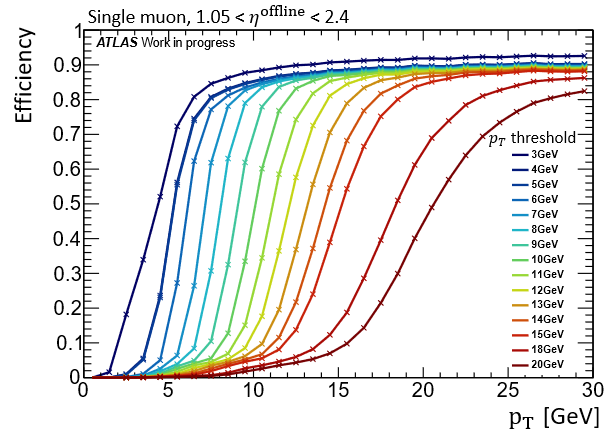
\includegraphics[clip, width=12cm]{fig/4/v07_15_Eff.png}
  \caption{<差し替え>シミュレーションデータをトレーニングに使用した機械学習を用いて作成した CW の 15 段階の閾値における Turn-on curve。}
  \label{fig:15Eff_CW_Simu}
\end{figure}

\begin{figure}[tb]
  \centering
  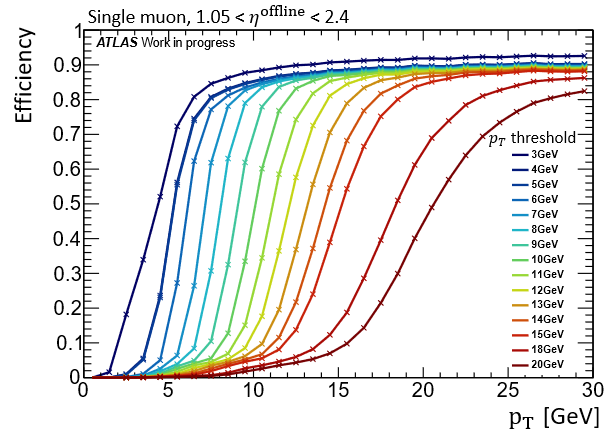
\includegraphics[clip, width=12cm]{fig/4/v07_15_Eff.png}
  \caption{<差し替え>2018年 Run-2 のデータをトレーニングに使用した機械学習を用いて作成した CW の 15 段階の閾値における Turn-on curve。}
  \label{fig:15Eff_CW_Data}
\end{figure}

\begin{figure}[tb]
  \centering
  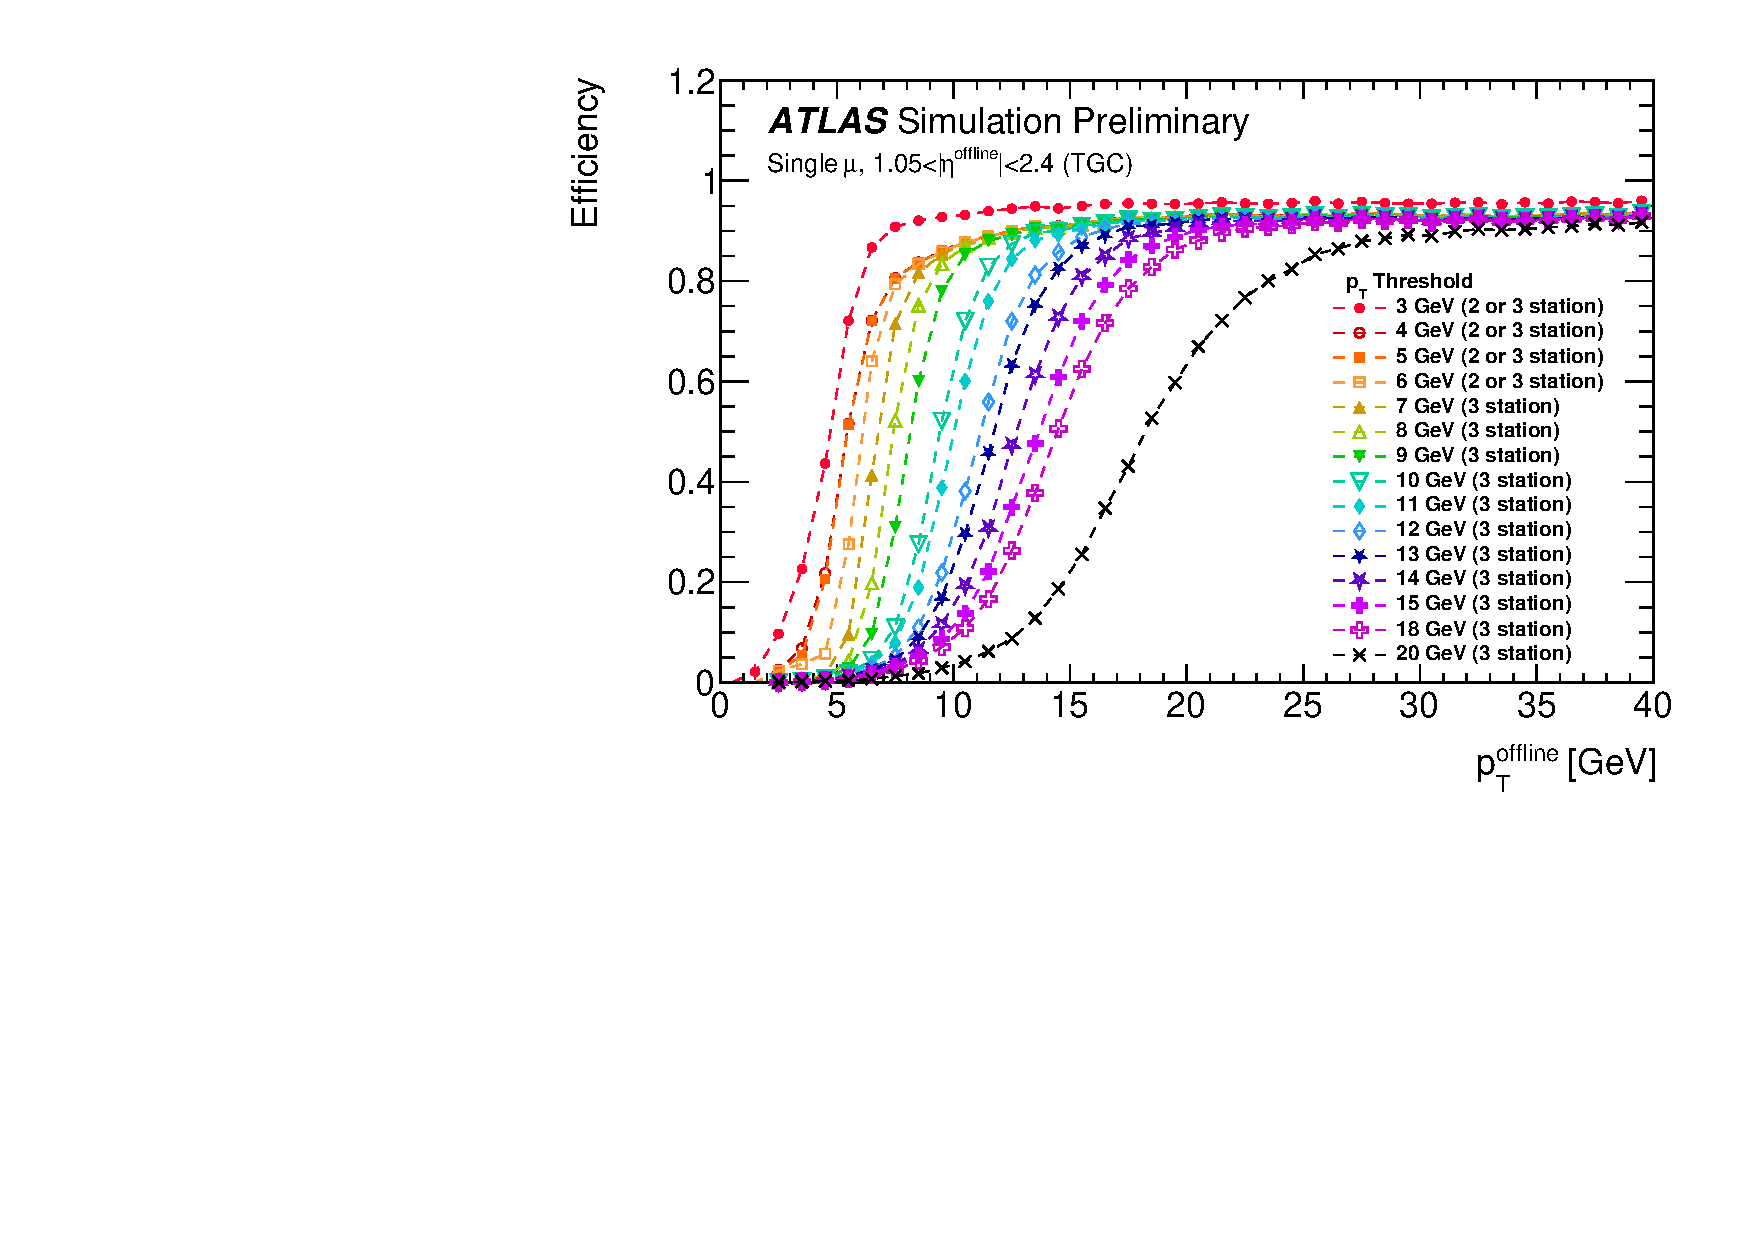
\includegraphics[clip, width=12cm]{fig/3/PLOT-TRIG-2020-01-fig1.pdf}
  \caption{2022年 Run-3 で使用した5段階閾値のTurn-on curve。シングルミューオンのシミュレーションサンプルに対してのトリガー効率を示している。}
  \label{fig:Run3_15_MC5}
\end{figure}

\begin{figure}[tb]
  \centering
  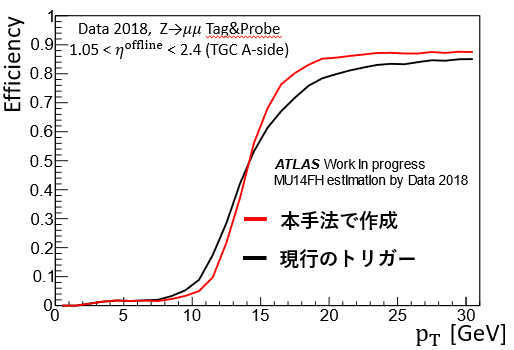
\includegraphics[clip, width=12cm]{fig/4/hikaku_v05_v06.png}
  \caption{v05v06}
  \label{fig:v05v06}
\end{figure}

\begin{figure}[tb]
  \centering
  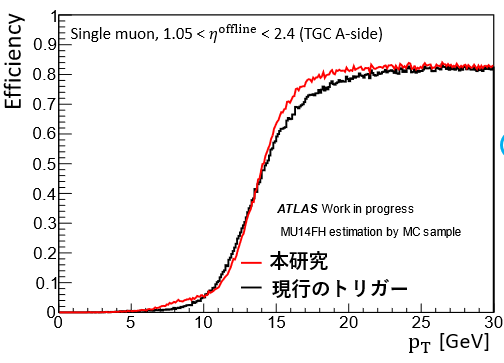
\includegraphics[clip, width=12cm]{fig/4/hikaku_v05_v07.png}
  \caption{v05v07}
  \label{fig:v05v07}
\end{figure}

\begin{figure}[tb]
  \centering
  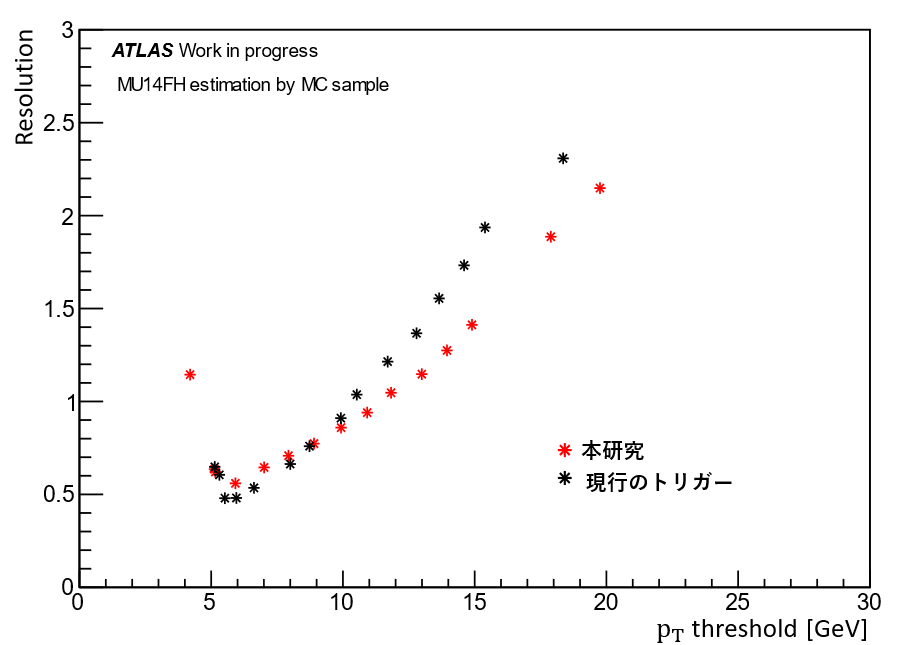
\includegraphics[clip, width=12cm]{fig/4/resolution_v07_v05.png}
  \caption{Resolutionv07v05}
  \label{fig:Resolution_v07v05}
\end{figure}

\begin{figure}[tb]
  \centering
  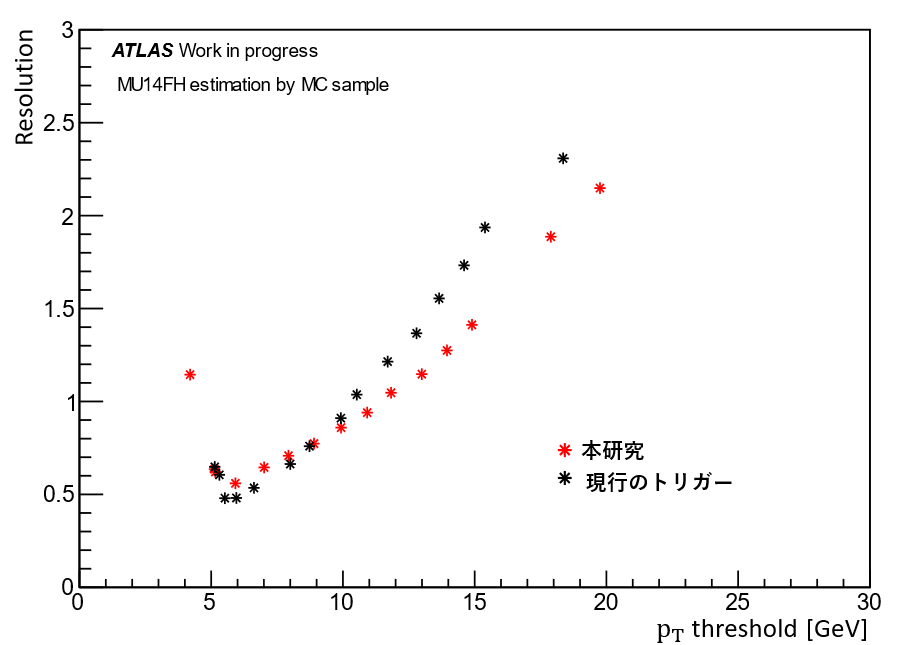
\includegraphics[clip, width=12cm]{fig/4/resolution_v07_v05.png}
  \caption{Resolutionv06v05}
  \label{fig:Resolution_v06v05}
\end{figure}

さらに、TGC チェンバーごとにトリガー効率の評価を行う。
\begin{figure}[tb]
  \centering
  \rule{8cm}{6cm}
  %\includegraphics[clip, width=14cm]{}
  \caption{チェンバーごとのEfficiency (1-48)}
  \label{fig:fit_def}
\end{figure}

次に、本手法で作成した CW を使用したときのトリガーレートの評価を行う。トリガーレートとは、実験データにおけるトリガーが発行された事象数である。ここでは HLT でのトリガー発行のバイアスを防ぐために、L1 Trigger のみを要求し、HLT は passthrough のトリガーである 「HLT$\_$noalg$\_$L1MU20」を要求する。

図\ref{fig:Ratev05v06} は 2016 年で取得されたデータを用いて算出したトリガーレートの $\eta$ 依存性である。

\begin{figure}[tb]
  \centering
  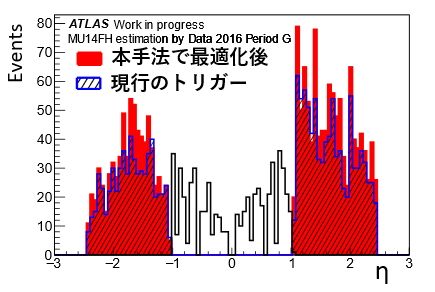
\includegraphics[clip, width=12cm]{fig/4/rate_v05_v06.png}
  \caption{ratev05v06}
  \label{fig:Ratev05v06}
\end{figure}

\subsection{ミューオン電荷に対するトリガー性能の評価}

\section{Run-3 に対するトリガー性能の評価}
2022 年 Run-3 のデータを用いてトリガー効率の評価を行う。
\begin{figure}[tb]
  \centering
  \rule{8cm}{6cm}
  \caption{Efficiency}
  \label{fig:fit_def}
\end{figure}

次に、本手法で作成した CW を使用したときの Run-3 におけるトリガーレートの評価を行う。
2022 年 Run-3 のデータを用い、トリガーには「」を要求する。
図\ref{fig:Run-3_rate}に$p_T$ 閾値が 8 GeV から 20 GeV までの 10 段階のトリガーレートを示す。
\begin{figure}[tb]
  \centering
  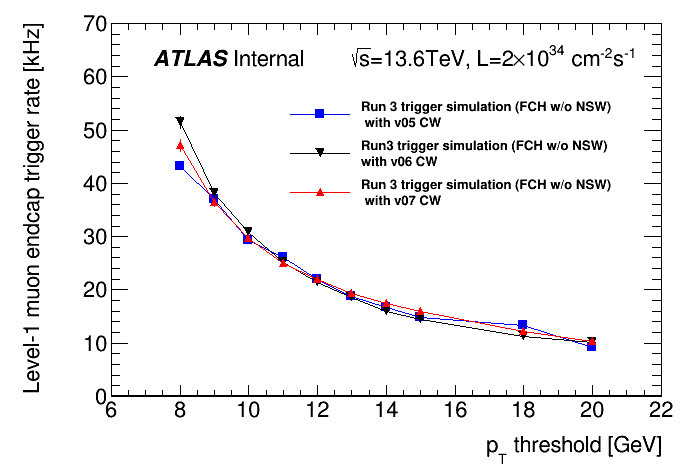
\includegraphics[clip, width=14cm]{fig/5/l1mue_rate_run3.png}
  \caption{Rate}
  \label{fig:Run-3_rate}
\end{figure}









